\documentclass[a4paper, 12pt]{report}
\usepackage[T2A]{fontenc} 
\usepackage[utf8]{inputenc}
\usepackage[english,russian]{babel} 
\usepackage{amsmath,amsfonts,amssymb,amsthm,mathtools}
\usepackage[left=2cm,right=2cm,top=2cm,bottom=2cm,bindingoffset=0cm]{geometry}
\usepackage{graphicx}
\usepackage[linesnumbered,boxed]{algorithm2e}
\usepackage{verbatim}

\newenvironment{Proof} 
{\par\noindent{$\blacklozenge$}}
{\hfill$\scriptstyle\boxtimes$} 

\newenvironment{example} 
{\par\noindent{\textsc{\textbf{Пример}.}}} 
{\hfill$\scriptstyle\Box$} 

\newtheorem*{theorem}{Теорема} 
\newtheorem*{corollary}{Следствие}
\newtheorem*{lemma}{Лемма}

\newcommand{\RNumb}[1]{\uppercase\expandafter{\romannumeral #1\relax}}
\newcommand{\Rm}{\mathbb{R}}
\newcommand{\Cm}{\mathbb{C}}
\newcommand{\I}{\mathbb{I}}
\newcommand{\N}{\mathbb{N}}
\newcommand{\Z}{\mathbb{Z}}
\newcommand{\Q}{\mathbb{Q}}

\title{\textbf{\Huge{Методы вычислений}}\\Лабораторная работа 4\\«Классические итерационные методы решения СЛАУ»\\Выполнила Николаева Ксения, 9 группа}
\date{} 

\begin{document}
    \maketitle

    \textbf{\Huge{Постановка задачи}}\\\\
    В данной лабораторной работе рассматриваются классические итерационные методы решения систем линейных алгебраических уравнений (СЛАУ). Необходимо написать и отладить программу на языке C++ для численного решения системы уравнений $Ax = b$ с квадратной матрицей порядка $n$.
Для решения поставленной задачи реализовать два метода:\\
1. Метод Якоби\\
2. Метод релаксации. Рассмотреть три случая: $\omega = 0.5$, $\omega = 1$ (это метод Гаусса-Зейделя), $\omega = 1.5$.


Задать параметры:
\begin{itemize}
    \item $n = 1000$
    \item $\varepsilon = 10^{-7}$
    \item $k_{max} = 1000$
\end{itemize}

Для проведения вычислительного эксперимента необходимо сгенерировать симметрическую матрицу $A$ с диагональным преобладанием (матрица генерируется один раз и используется для всех заданий). СЛАУ формируется следующим образом:

\begin{enumerate}
    \item Заполнить нижнюю треугольную часть матрицы $A$ (элементы $a_{ij}$, где $i > j$) случайными целыми числами из диапазона от $100$ до $1000$.
    \item Заполнить верхнюю треугольную часть матрицы $A$ симметрично нижней части.
    \item Заполнить диагональ матрицы. В качестве диагонального элемента $a_{ii}$ выбрать случайное целое число из интервала $\left[\sum_{j \neq i} |a_{j}| + m, \sum_{j \neq i} |a_{j}| + 10m\right]$, где $m$ — номер студента в списке рейтинга подгруппы.
    \item Задать точное решение $x = (m, m + 1, \ldots, m + n - 1)^T$ и образовать правую часть $b$ как $b = Ax$.
\end{enumerate}

Задать начальное приближение $x^{(0)}$, которое должно быть одинаковым для всех заданий.

\newpage
\textbf{\Huge{Краткие теоретические сведения}}\\\\
\textbf{Метод Якоби} является классическим итерационным методом для решения систем линейных уравнений. Он основывается на разложении матрицы $A$ на компоненты, что позволяет выразить каждую переменную через другие. Формула обновления переменной $x_i$ имеет следующий вид:

\[
x_i^{(k+1)} = \frac{1}{a_{ii}} \left( b_i - \sum_{j=1}^{i-1} a_{ij} x_j^{(k)} - \sum_{j=i+1}^{n} a_{ij} x_j^{(k)} \right), \quad i = 1, \ldots, n, \quad k = 0, 1
\]

\textbf{Метод релаксации} улучшает сходимость метода Якоби за счет введения параметра релаксации $\omega$:

\[
x_i^{(k + 1)} = (1 - \omega)x_i^{(k)} + \omega \dfrac{1}{a_{ii}} \left( b_i - \sum_{j=1}^{i-1} a_{ij} x_j^{(k + 1)} - \sum_{j=i+1}^{n} a_{ij} x_j^{(k)} \right), \quad i = 1, \ldots, n, \quad k = 0, 1
\]

\textbf{ля метода релаксации}:
- В случае $\omega = 1$ метод переходит в метод Гаусса-Зейделя.
- Для выбора значения $\omega$ можно использовать различные подходы, чтобы обеспечить более быструю сходимость.

\textbf{Погрешности в вычислениях} делятся на абсолютные и относительные:
\begin{itemize}
    \item Абсолютная погрешность — это разность между истинным и вычисленным значениями.\\
Если обозначить точное решение как $x$ и приближенное решение как $x^{(q)}$, то абсолютная погрешность может быть вычислена следующим образом: $||x - x^{(q)}||_{\infty}$
    \item Относительная погрешность — отношение абсолютной погрешности к истинному значению.
    
\end{itemize}


   \newpage
   \textbf{\Huge{Листинг программы с комментариями}}\\\\
   \begin{verbatim}
#include <bits/stdc++.h>
using namespace std;

const int N = 1000;
const int MAX_ITER = 1000;
const double EPS = 1e-7;
double omega_values[] = {0.5, 1.0, 1.5};

int n = 1000;
int m = 8;

vector<vector<long double>> A;
vector<long double> b, exact_x, approx_x;

/// Создание матрицы А
void createMatrix() {
    srand(time(0));
    A.assign(n, vector<long double>(n, 0));

    for (int i = 0; i < n; ++i) {
        for (int j = i + 1; j < n; ++j) {
            A[i][j] = rand() % 201 - 100;
        }
    }
    for (int i = 0; i < n; ++i) {
        for (int j = 0; j < i; ++j) {
            A[i][j] = A[j][i];
        }
    }
    for (int i = 0; i < n; ++i) {
        int sum = 0;
        for (int j = 0; j < n; ++j) {
            if (i != j) sum += abs(A[i][j]);
        }
        A[i][i] = sum + rand() % (10 * m + 1);
    }
}

/// Создание вектора b
void createB(int n) {
    b.assign(n, 0);
    for (int i = 0; i < n; ++i) {
        for (int j = 0; j < n; ++j) {
            b[i] += A[i][j] * exact_x[j];
        }
    }
}

/// Вывод результатов
void printResults(int n, int iter, const vector<long double>& x, const vector<long double>& x_prev) {
    cout << "Results after " << iter << " iterations:\n";
    cout << "Approximate solution (first and last 5 values):\n";
    for (int i = 0; i < 5; ++i)
        cout << "x[" << i << "] = " << fixed << setprecision(20) << x[i] << '\n';
    cout << "...\n";
    for (int i = n - 5; i < n; ++i)
        cout << "x[" << i << "] = " << fixed << setprecision(20) << x[i] << '\n';

    /// Подсчет абсолютной погрешности
    long double max_diff = 0, max_exact = 0;
    for (int i = 0; i < n; ++i) {
        max_diff = max(max_diff, abs(exact_x[i] - x[i]));
    }
    cout << "Absolute error: " << scientific << setprecision(15) << max_diff << "\n";

    for (int i = 0; i < n; ++i) {
        max_diff = max (max_diff, x[i] - x_prev[i]);
        max_exact = max (max_exact, x[i]);
    }
    cout << "Additional result: " << scientific << setprecision(15) << max_diff / max_exact << "\n\n";
}

/// Метод Якоби
void jacobiMethod(int n) {
    vector<long double> x_prev(n, 0);
    approx_x.assign(n, 0);
    int iter = 0;

    while (iter < MAX_ITER) {
        for (int i = 0; i < n; ++i) {
            long double sigma = 0;
            for (int j = 0; j < n; ++j) {
                if (j != i) sigma += A[i][j] * x_prev[j];
            }
            approx_x[i] = (b[i] - sigma) / A[i][i];
        }

        long double max_diff = 0, max_x = 0;
        for (int i = 0; i < n; ++i) {
            max_diff = max(max_diff, abs(approx_x[i] - x_prev[i]));
            max_x = max(max_x, abs(approx_x[i]));
        }
        if (max_diff / max_x < EPS) break;

        x_prev = approx_x;
        ++iter;
    }
    if (iter == MAX_ITER) {
        cout << "Jacobi Method: Exceeded maximum number of iterations.\n";
    }
    cout << "---------------------\n";
    cout << "Jacobi Method:\n";
    cout << "---------------------\n";
    printResults(n, iter, approx_x, x_prev);
}

/// Метод релаксации
void relaxationMethod(int n, double omega) {
    vector<long double> x_prev(n, 0);
    approx_x.assign(n, 0);
    int iter = 0;

    while (iter < MAX_ITER) {
        for (int i = 0; i < n; ++i) {
            long double sigma = 0;
            for (int j = 0; j < i; ++j) {
                sigma += A[i][j] * approx_x[j];
            }
            for (int j = i + 1; j < n; ++j) {
                sigma += A[i][j] * x_prev[j];
            }

            approx_x[i] = (1 - omega) * x_prev[i] + omega * (b[i] - sigma) / A[i][i];
        }

        long double max_diff = 0, max_x = 0;
        for (int i = 0; i < n; ++i) {
            max_diff = max(max_diff, abs(approx_x[i] - x_prev[i]));
            max_x = max(max_x, abs(approx_x[i]));
        }
        if (max_diff / max_x < EPS) break;

        x_prev = approx_x;
        ++iter;
    }
    if (iter == MAX_ITER) {
        cout << "Relaxation Method (omega = " << omega << "): Exceeded maximum number of iterations.\n";
    }
    cout << "---------------------------------------\n";
    cout << "Relaxation Method (omega = " << fixed << setprecision(1) << omega << "):\n";
    cout << "---------------------------------------\n";
    printResults(n, iter, approx_x, x_prev);
}

int main() {
    freopen("output.txt", "w", stdout);

    createMatrix();

    exact_x.resize(n);
    for (int i = 0; i < n; ++i) {
        exact_x[i] = m + i;
    }

    createB(n);

    /// Вывод начального приближения
    cout << "Initial approximation (first and last 5 values):\n";
    for (int i = 0; i < 5; ++i) cout << "x[0][" << i << "] = 0\n";
    cout << "...\n";
    for (int i = n - 5; i < n; ++i) cout << "x[0][" << i << "] = 0\n";

    /// Вывод точного решения
    cout << "Exact solution (first and last 5 values):\n";
    for (int i = 0; i < 5; ++i) cout << "x_exact[" << i << "] = " << exact_x[i] << '\n';
    cout << "...\n";
    for (int i = n - 5; i < n; ++i) cout << "x_exact[" << i << "] = " << exact_x[i] << '\n';

    jacobiMethod(n);

    for (double omega : omega_values) {
        relaxationMethod(n, omega);
    }

    return 0;
}
   \end{verbatim}
   \newpage
   \textbf{\Huge{Результаты}}\\\\
   $\bullet$ Результат работы метода Якоби\\
   \begin{center}
        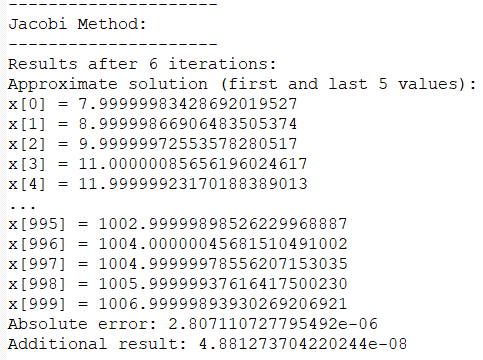
\includegraphics[scale = 0.7]{pic9.png}
   \end{center}
   $\bullet$ Результат работы метода релаксации при $\omega = 0.5$\\
   \begin{center}
        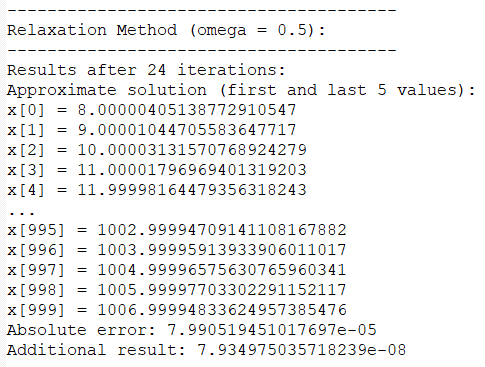
\includegraphics[scale = 0.7]{pic10.png}
   \end{center}
   $\bullet$ Результат работы метода релаксации при $\omega = 1.0$\\
   \begin{center}
        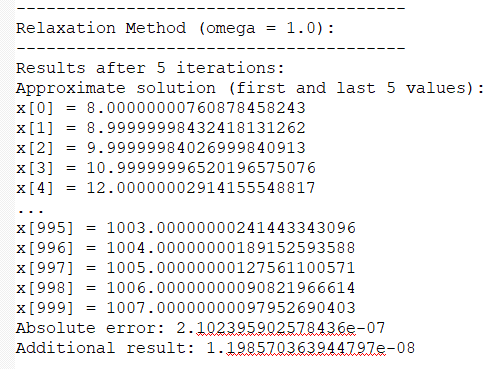
\includegraphics[scale = 0.7]{pic11.png}
   \end{center}
   $\bullet$ Результат работы метода релаксации при $\omega = 1.5$\\
   \begin{center}
        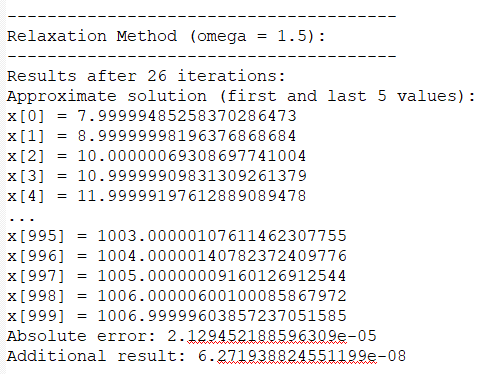
\includegraphics[scale = 0.7]{pic12.png}
   \end{center}
   

    \newpage
   \textbf{\Huge{Выводы}}\\\\
      $\bullet$  В ходе лабораторной работы были протестированы методы Якоби и релаксации для решения системы линейных уравнений. Метод Якоби показал более быструю сходимость по сравнению с методом релаксации, что делает его более предпочтительным для данной задачи.\\
      $\bullet$  Результаты показали, что выбор параметра $\omega$ в методе релаксации критически важен для достижения хорошей сходимости. Оптимальное значение $\omega = 1$ обеспечивало наилучшие результаты, в то время как слишком высокие или низкие значения приводили к замедлению процесса.\\
      $\bullet$ Абсолютные ошибки, полученные при использовании методов, свидетельствуют о высокой точности полученных приближенных решений по сравнению с точными значениями. Это подтверждает возможность применения данных методов для практических задач, требующих высокой точности.\\
      $\bullet$ Полученные результаты подчеркивают необходимость дальнейшего изучения и оптимизации методов решения линейных систем, включая адаптацию алгоритмов для различных типов задач и улучшение их вычислительной эффективности.\\
   
\end{document}


